\documentclass[letterpaper,12pt]{article}
\usepackage{amsmath}  % improve math presentation
\usepackage{graphicx} % takes care of graphic including machinery
\usepackage{mathrsfs}


\usepackage[final]{hyperref} % adds hyper links inside the generated pdf file
\hypersetup{
	colorlinks=true,       % false: boxed links; true: colored links
	linkcolor=blue,        % color of internal links
	citecolor=blue,        % color of links to bibliography
	filecolor=magenta,     % color of file links
	urlcolor=blue         
}

\title{Fourth Assignment for Computational Physics}
\date{\today}
\author{Xinyu Liu}


\begin{document}
\maketitle
\tableofcontents

\newpage

\section{My Github Page URL}
\url{https://github.com/rising1227/phys-ga2000}

\section{Problem 1: Exercise 5.9 of Newman}

The Associated Code for this part is ps4-1.py.

We wrote a standard code to calculate the integration with gaussian quadrature approximation with N=50. The relation between heat capacity and temperature is($V=1000cm^2,\rho_{numberdensity} = 6.022*10^{26},\theta_D = 428K$):

\begin{table}[!h]
    \centering
    \caption{Heat capacity wrt temperature}
    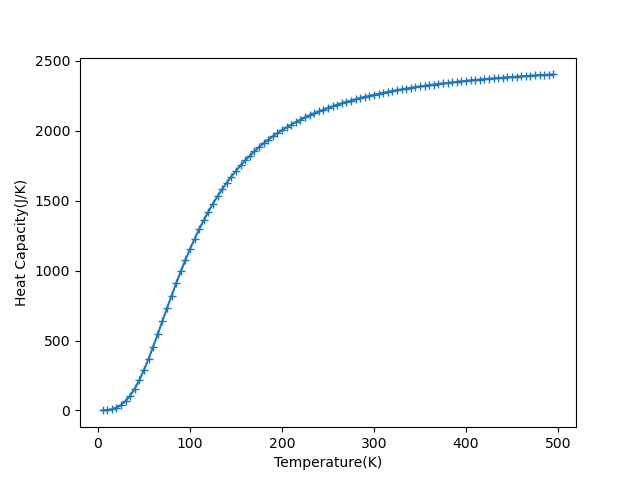
\includegraphics[width=12cm]{ps4-1-2.png}
\end{table}%

After that, we test the convergence of numerical integration with large N. We calculate the heat capacity at 300K with different N. The result is 2256.73598491, 2256.73598491, 2256.73598491, 2256.73598491, 2256.73598491, 2256.73598491, 2256.73598491, which is exactly the same. This shows that N=10 can already lead to very good approximation for the integration.





\section{Problem 2: Exercise 5.10 of Newman}

The Associated Code for this part is ps4-2.py

The theoretical derivation for the period is simple, assume that the oscillator has the amplitude a, with the conservation of energy, we have:

\begin{equation}
    V(a) = \frac{1}{2}m(\frac{dx}{dt})^2 + V(x)
\end{equation}

So that:

\begin{equation}
    dt = \sqrt{2m}\frac{dx}{\sqrt{V(a)-V(x)}}
\end{equation}

For the movement from 0 to a, which is one forth of a period:

\begin{equation}
    T/4 = \int_0^a dt = \int_0^a \sqrt{2m}\frac{dx}{\sqrt{V(a)-V(x)}}
\end{equation}

So that the period T satisfies:

\begin{equation}
    T = \sqrt{8m} \int_0^a \frac{dx}{\sqrt{V(a)-V(x)}}
\end{equation}

Then we assume that the potential energy for the system is:

\begin{equation}
    V(x) = x^4
\end{equation}

Now,
\begin{equation}
    T = \sqrt{8m} \int_0^a \frac{dx}{\sqrt{a^4-x^4}}
\end{equation}

This integration can be calculated using gaussian quadrature. We can plot a plot for the periodicity wrt the amplitude:


\begin{table}[!h]
    \centering
    \caption{Period wrt Amplitude}
    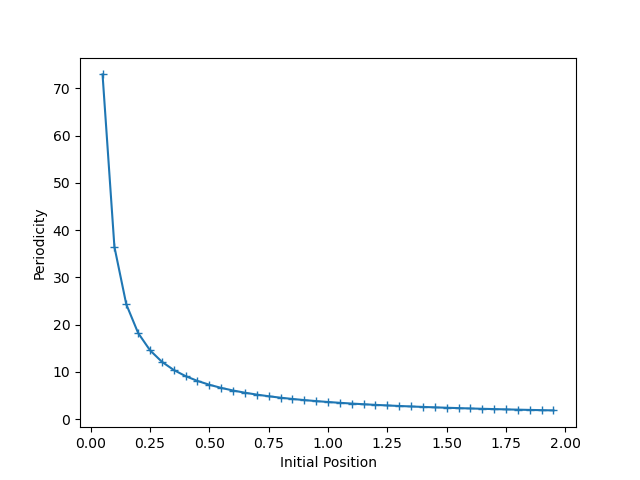
\includegraphics[width=12cm]{ps4-2-2.png}
\end{table}%

\newpage

We indeed find that the period diverge when amplitude A goes to 0 and the period go to 0 when amplitude goes to infinity. This is reasonable since the period is a constant for harmonic oscillator with a $x^2$ potential. If the amplitude is very small, the amplitude and the restoring force for $x^4$ field is much smaller than $x^2$ field, thus the period is longer the smaller a is. In the contrary, if the amplitude is very large, the amplitude and the restoring force for $x^4$ field is much larger than $x^2$ field, thus the period is shorter the larger a is.



\section{Problem 3: Exercise 5.13 of Newman}

The Associated Code for this part is ps4-3.py

We calculate the Hermite function by doing induction. In order to compute the hermite function faster, we calculate the mathematical form of Hermite function in the beginning. This result is stored in the array named "array" at the beginning of ps4-3.py. We can then calculate the wavefunction for different N. We then plot the wave function for n=0,1,2,3 and n=10.

\begin{table}[!h]
    \centering
    \caption{Wavefunction for harmonic oscillatore for n = 0,1,2,3}
    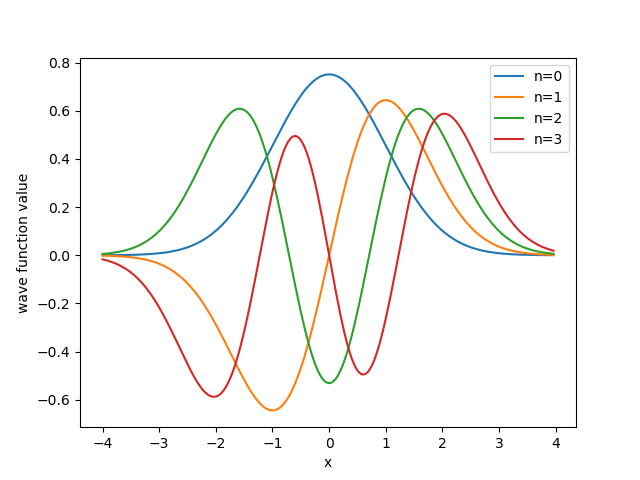
\includegraphics[width=10cm]{ps4-3-1.png}
    \label{plot}%
\end{table}%

\begin{table}[!h]
    \centering
    \caption{Wavefunction for harmonic oscillatore for n = 30}
    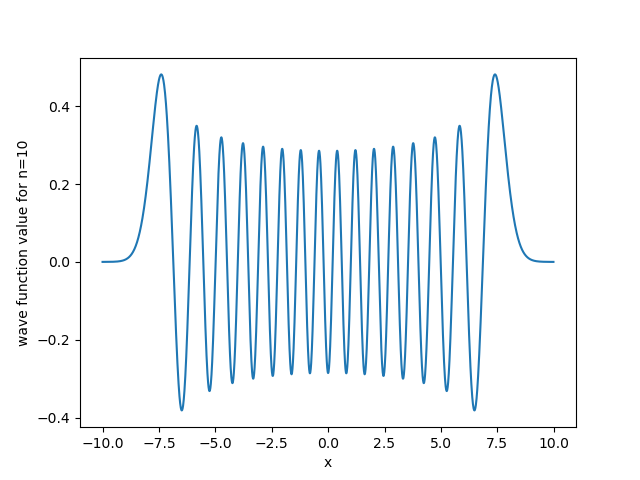
\includegraphics[width=10cm]{ps4-3-2.png}
    \label{plot}%
\end{table}%
\newpage

We then use the gaussian quadrature to calculate the uncertainty for position for each eigenstate n. This is done in the function "uncertainty" in ps4-3.py. We found that the uncertainty of n=5 is 2.3452078799117158. We do the similar calculation with Gauss-Hermite quadrature and this is done in the function "uncertaintyH" in ps4-3.py, we found that the result is 2.3452078799117246.

The Gauss-Hermite quadrature method can theoretically provide the exact result since the function apart from $e^{-x^2}$ is polynomial. In fact we found that there's still slight computational error due to rounding effect in the python program. 














\end{document}